\documentclass{article}

\usepackage{multirow}
\usepackage{graphicx}
\usepackage{tikz}
\usepackage{placeins}
\usepackage{url}
\usepackage{float}
\usepackage{xcolor}
\usepackage[sorting=none,maxbibnames=4]{biblatex}

\definecolor{l_red}{HTML}{F8CECC}
\definecolor{l_orange}{HTML}{FFE6CC}
\definecolor{l_yellow}{HTML}{FFF2CC}
\definecolor{l_green}{HTML}{D5E8D4}
\definecolor{d_red}{HTML}{B85450}
\definecolor{d_orange}{HTML}{D79B00}
\definecolor{d_yellow}{HTML}{D6B656}
\definecolor{d_green}{HTML}{82B366}

\addbibresource{references.bib}

\title{Design and Simulation of a USB 2.0 Transceiver in SystemVerilog}
\author{Andrew Lu, Jiayi Liu, Leo Lesmes, Nhan Do \\
\small \url{https://github.com/leo-les/usb-transceiver}\autocite{usb-transceiver}
}

\graphicspath{{images/}}

\begin{document}
\maketitle

\section{Technical}
\subsection{Overview}
The USB Transceiver covers the physical (PHY) layer of USB communication, bridging the digital data used by a host controller (computers, smartphones, etc.) with the electrical signals sent through USB wires to a device controller (mouses, keyboards, flash drives, etc.). In other words, the transceiver acts as a bidirectional translator between digital logic (1s and 0s) and analog voltage levels on its two differential data wires, D+ and D-.

\begin{figure}[htp]
    \centering
    \includegraphics[width=8cm]{asic_functional_blocks}
    \caption{ASIC Functional Blocks\autocite{intel2001utmi}}
    \label{fig:asic}
\end{figure}

Our project aimed to simulate the behavior of a USB 2.0 Low Speed Transceiver in SystemVerilog, which sends and receives data at 1.5 Mbps utilizing a 48 Mhz clock signal. To the left of the USB 2.0 Transceiver block is a Serial Interface Engine (SIE), which treats incoming data as packets and sends serial data to the transceiver. To the right of the block are D+/D- wires, connecting the transceiver to a device controller.

\begin{figure}[htp]
    \centering
    \includegraphics[width=12cm]{RTL}
    \caption{UTMI RTL Diagram}
    \label{fig:rtl}
\end{figure}

\newpage

The Register-Transfer Level (RTL) design above maps out all the modules implemented in SystemVerilog making up our transceiver. The top and bottom halves of the diagram consists of all the modules receiving from and transmitting data to the D+/D- wires, respectively. The top module, represented by the box encompassing all the modules, initializes all the modules and connects their signals to allow for a layer of abstraction from the individual modules.

\subsubsection*{Hardware \& Software}
Numerous pieces of software were used to help develop this project, along with multiple coding languages. The names of the products used, along with their purpose in the project, are listed below.

\begin{table}[htp]
    %\centering
    \hspace*{-0.15cm}
    \resizebox{\columnwidth}{!}{
    \begin{tabular}{ |l|l|l| } 
        \hline
        \multicolumn{1}{|c|}{\textbf{Type}} & \multicolumn{1}{c|}{\textbf{Name}} & \multicolumn{1}{c|}{\textbf{Purpose}} \\
        \hline
        \multirow{7}{6em}{Software} & Google Docs & Research/brainstorming, writing for proposal and check-ins \\
        & Figma & Research/brainstorming, and drafting diagrams \\ 
        & Draw.io & Used to create final diagrams and flowcharts \\ 
        & Google Slides & Slideshow software that the Final Presentation was created in. \\ 
        & Visual Studio Code & IDE used for coding the project and writing the final report. \\
        & Github & Project was hosted and shared \\ 
        & MyFPGA & In web-browser simulation tool for testing SystemVerilog code \\ 
        \hline
        \multirow{4}{6em}{Programming Language} & SystemVerilog & Language that the UTMI was written in \\ 
        & C++ &  \\
        & Makefile &  \\
        & LaTeX & Final project report (this document) was written in LaTeX \\
        \hline
\end{tabular}}

\caption{Products used to develop the project}
\label{table:1}
\end{table}

\subsubsection*{Division of Labor}
\textcolor{white}{} % Prevents section header from jumping to next page
Numerous pieces of software were used to help develop this project, along with multiple coding languages. The names of the products used, along with their purpose in the project, are listed below.

\begin{figure}[htp]
    \centering
    \includegraphics[width=12cm]{DOL}
    \caption{Division of Labor}
    \label{fig:dol}
\end{figure}

\newpage

\subsubsection*{Timeline}
We kept our project to a pretty strict timeline
\begin{figure}[H]
\centering
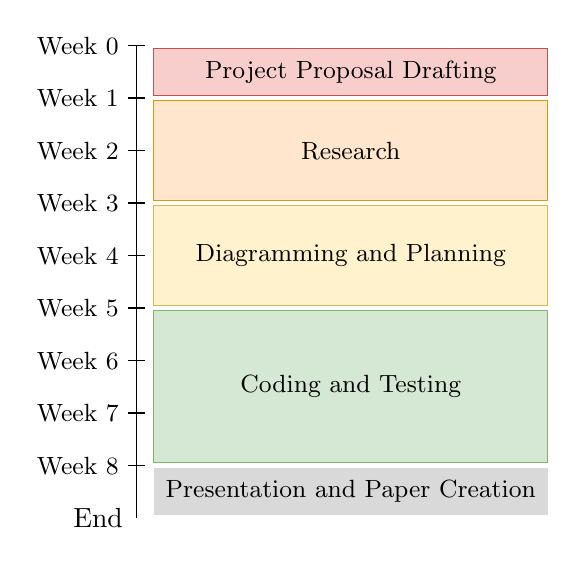
\begin{tikzpicture}
\draw (0,0) -- (0,9/1.5);

\foreach \y in {1,2,3,4,5,6,7,8,9}
\draw (3pt,\y cm/1.5) -- (-3pt,\y cm/1.5);

\draw (0,0) node[left=3/2pt] {End};

\draw (0,1/1.5) node[left=3pt] {\small Week 8};
\draw (0,2/1.5) node[left=3pt] {\small Week 7};
\draw (0,3/1.5) node[left=3pt] {\small Week 6};
\draw (0,4/1.5) node[left=3pt] {\small Week 5};
\draw (0,5/1.5) node[left=3pt] {\small Week 4};
\draw (0,6/1.5) node[left=3pt] {\small Week 3};
\draw (0,7/1.5) node[left=3pt] {\small Week 2};
\draw (0,8/1.5) node[left=3pt] {\small Week 1};
\draw (0,9/1.5) node[left=3pt] {\small Week 0};

\draw (0,8.5/1.5) node[minimum height=.9cm/1.5,minimum width =5cm,right=6pt, fill=l_red, draw = d_red] {\small Project Proposal Drafting};
\draw (0,7/1.5) node[minimum height=1.9cm/1.5,minimum width =5cm,right=6pt, fill =l_orange, draw =d_orange] {\small Research};
\draw (0,5/1.5) node[minimum height=1.9cm/1.5, minimum width =5cm,right=6pt, fill =l_yellow, draw = d_yellow] {\small Diagramming and Planning};
\draw (0,2.5/1.5) node[minimum height=2.9cm/1.5, minimum width =5cm,right=6pt, fill =l_green, draw = d_green] {\small Coding and Testing};
\draw (0,.5/1.5) node[minimum height=.9cm/1.5, minimum width =5cm,right=6pt, fill =gray!30] {\small Presentation and Paper Creation};


\end{tikzpicture}
\caption{Timeline}
\label{fig:timeline}
\end{figure}


\subsection{Design}
\paragraph{RX State Machine:}
The RX State Machine monitors the reception of data from the differential data wires, primarily checking for the
\paragraph{TX State Machine:}
The TX State Machine controls the transmitting process. It organizes the states in which the data is loaded and sent. It controls when the data is loaded into the shift register and waits until a 8 bits (1 byte) is present and then serially shifts out the bits. The state machine ensures data is smoothly transferred from an SIE to the differential data wires and protects against cases in which data might be corrupted or imprecisely loaded. 
\paragraph{DPLL:}
The Digital Phase Locked Loop (DPLL) module generates a pulse at the middle of each incoming clock signal when the transceiver is receiving signals from D+/D-, ensuring clock synchronization of all the modules with the incoming signals. The pulse is propagated to the rest of the receiving modules.
\paragraph{EOP Detector:}
The EOP detector is used to detect the End Of Packet signal, or EOP, on the receiving side of the transceiver. When the receiver detects an EOP, it knows that there is no more incoming data. EOP is signalled by two clock cycles of the SE0 state, where both data lines are pulled low, followed by the low-speed idle state, where D+ is 1 and D- is 0. 
\paragraph{NRZI Decoder/Encoder:}
The USB 2.0 protocol transmits and receives data through the NRZI encoding schematic. Instead of encoding data through 0s and 1s on the data line, data is encoded through the presence or absence of edges on the data line, with both the receiver and transmitter operating at the same clock frequency. A zero is encoded in this new line of data through a signal transition, either from 0 to 1, or 1 to 0, and a 1 is encoded through a constant signal level. 
When decoding an encoded signal, we know that edges on the incoming data line encode a 0, and no change in the data line encodes a 1. 
\paragraph{Bit Stuffing/Unstuffing:}
Though the NRZI protocol can be efficient, it also comes with downsides. Because a 1 is encoded with an unchanging signal, the high frequency transmitter and receiver are at risk of desynchronization when too many 1s are transmitted in a row. Thus, the concept of bit stuffing was invented. Whenever six 1s are transmitted in a row on a data line, a 0 is ``stuffed'' into the data sequence, following the six 1s, which manifests as a level transition in the data. This stuffed bit acts as a re-synchronization signal for the receiver and transmitter, ensuring a stable communication connection. 
On the receiving end, the stuffed bits must be removed to recover the original data, which is accomplished through the use of a bit unstuffer. An unstuffer implements the reverse of the stuffing protocol, ignoring the stuffed bit that always follows six consecutive 1s. The unstuffer can also be used to detect transmission errors if it receives data that has not been bit stuffed.

\begin{figure}[htp]
    \centering
    \includegraphics[width=10cm]{nrzi_stuffing.png}
    \caption{Bit Stuffing and NRZI Encoding}
    \label{fig:bs/nrzi}
\end{figure}

\paragraph{SIPO Register:} 
SIPO (Serial-in-parallel-out): SIPO shift register is a sequential logic device that can store and shift data bits. "Serial-in" means that the data is entered into the register one bit at a time. "Parallel out" means that data is accessed simultaneously.

\paragraph{PISO Register:} 
PISO (Parallel-in-serial-out): PISO shift register accepts parallel data and output serial data. The data is loaded into the register simultaneously through multiple input lines. The output comes out as serial data (bit by bit).


\pagebreak

\subsection{Simulation}

\subsubsection*{Testing \& Benchmarks}
\begin{itemize}
    \item USB transceiver transmits and receives data as stated in our proposal.
    \item Individual modules were tested and verified with testbenches. SystemVerilog testbenches were created and run using Makefile. For the final simulation, we used the ecelabs.io website to get our design simulated and collect data from the generated waveforms.
    \item Predetermined bytes were used as test cases. After analyzing the waveforms, we confirmed that it correctly decodes and unstuffs the data for receiving as well as stuffs and encodes the data for transmitting.
\end{itemize}

\subsubsection*{Waveform Results}

\begin{figure}[htp]
    \centering
    \includegraphics[width=12cm]{sim_tx_sync.png}
    \caption{Transmitting 8'b00000001 (SYNC) Byte Waveform}
    \label{fig:t1}
\end{figure}

\begin{figure}[htp]
    \centering
    \includegraphics[width=12cm]{sim_tx_00010101.png}
    \caption{Transmitting 8'b00010101 Byte Waveform}
    \label{fig:t2}
\end{figure}

\begin{figure}[htp]
    \centering
    \includegraphics[width=12cm]{sim_tx_01111111.png}
    \caption{Transmitting 8'01111111 Byte Waveform}
    \label{fig:t3}
\end{figure}

\begin{figure}[htp]
    \centering
    \includegraphics[width=12cm]{sim_rx_01010101.png}
    \caption{Receiving 8'b01010101 Byte Waveform}
    \label{fig:r1}
\end{figure}

\begin{figure}[htp]
    \centering
    \includegraphics[width=12cm]{sim_rx_11111101}
    \caption{Receiving 8'b11111101 Byte Waveform}
    \label{fig:r}
\end{figure}

\newpage
\subsubsection*{Operation Documentation}
The USB transceiver is packaged into a top-level usb-transceiver.sv SystemVerilog file. At a high level, it is similar to a Python or C++ class, with abstracted inputs and outputs that the user can interface with to control the whole module, and a hardware analogue would be a physical USB transceiver with input and output pins. 
To send data to the transceiver, simply pulse the input D+and D- with whatever signal you want to send the transceiver, with D- being the logical NOT of D+. The received data will appear in the data-in shift register after it is received. 
To transmit data using the transceiver, use the transmit enable and transmit valid pins to load in data to the transmission shift register, which will first send a SYNC signal, confirming the start of transmission and then shift out each bit, stuffed and encoded, to the output D+ and D- wires, where D- is the inverse of D+.

\subsubsection*{Expansion/Next Steps}
For our next steps, we were inspired by a post-presentation question to implement our transceiver on an actual USB device. We would have to implement the actual serial interface logic, which manages packet transfers, handshakes, and interfaces with the device hardware. Following this, the device itself would be implemented in hardware with SystemVerilog, which could be a mouse, keyboard,  or any other kind of USB peripheral. Finally, we would flash this onto an FPGA and test our USB device by connecting through PMOD or wires to a USB port, allowing us to put our device and transceiver to use. 

\section{Reflection}
\subsection*{Learning Outcomes}
Building this from the ground up forced us to apply our digital design skills. Besides that, it also required us to find reliable sources and read technical documentations. These are crucial skill sets which can be applied to our future ECE courses and career paths. We also significantly improved our testbench writing by figuring out how to generate the Makefile, create the simulations, and analyze the results. Ultimately, we understand the technical concepts of a USB transceiver design. As for a potential continuing of this project in Intro II, we could implement peripheral interfaces like the SIE and/or test a hardware implementation of the USB transceiver.

\newpage
\subsection*{Preferences}
\paragraph{Andrew:}
I enjoyed implementing all of the logic behind the transceiver in SystemVerilog and producing the waveform outputs of our working modules, though I disliked the tedious process of debugging the modules with testbenches.
\paragraph{Jiayi:}
Through this project, I learned more about what digital design looks like at a professional level. It requires precise timing and meeting hardware and protocol specifications, which can be tedious at times. However, the system-level design is interesting and fun. I learned that I enjoy designing and conceptually building digital systems, but I do not like the low level details of actually implementing it.
\paragraph{Leo:} I also gained a lot more interest in exploring Analog Design from this project. 
\paragraph{Nhan:}
After working on this project, I found my interest in working with digital designs. I hope to have more opportunities to get involved in digital projects in the future. I would also like to gain a deeper understanding of digital peripherals and communication. 
\subsection*{Challenges}
\subparagraph{}The main challenge of the project was finding and understanding all the technical specifications for what we were trying to design. We had to spend a significant amount of time on doing research on the Internet, reading articles, and finding other reliable sources. If challenging topics were encountered, our team discussed them together and tried to understand them together. 

Another challenge that we encountered was establishing a large project with a newly learned language. To overcome the difficulties, we had to read numerous articles and follow many guidelines to get the right direction. Although debugging costed us a considerable amount of time, we successfully got out design simulated and collected the results. 

When it came to scheduling, it was difficult to manage the timeline over a long period as we had other to-dos to finish. However, our team usually met whenever a member ran into issues and tried to solve the problems. When everybody had finished with their modules, we worked together on the top module and implemented our parts into the final design. After the design was created, results analysis jumped in. Eventually, all the important milestones that we set in the beginning were completed as the team effectively cooperated with each other. 

\newpage
When it came to actually coding the project, the hardest part was integrating all of the modules together and passing all of the test cases. As each teammate self-design their own modules, it took us some time to merge all the parts together and make them work effectively. At the end of the design process, our team worked together on the FSMs and the top module. Everyone understood their parts and explained them to everyone, which greatly accelerated our progress.

\nocite{murphy2014usb101}
\printbibliography
\end{document}